\chapter{Solution to One-Variable Equation}

There are variety of ways to solve the scalar function $f(x)=0$ for independent variable $x$, the most intuitive of which being deriving its analytical solution in the form of $x=\cdots$. However, in many cases the general analytical solution of $x$ may not exist or be very difficult to achieve. To address this problem, many numerical analysis based methods have been developed to obtain (an approximation of) the solution effectively and efficiently.

This chapter discusses these numerical methods as well as their convergence and computational burden. 

\section{Problem Formulation}

Let $f(x)=0$ be a scalar function, where $f(x)$ is continuous. There is at least one solution to $f(x)=0$, namely $p$, and $p\in \left[a, b\right]$. The target is find (one of the) value of $p$. A demonstrative plot is given in Fig. \ref{fig:p5:onevarproblemformulation}.

\begin{figure}[htbp]
\centering
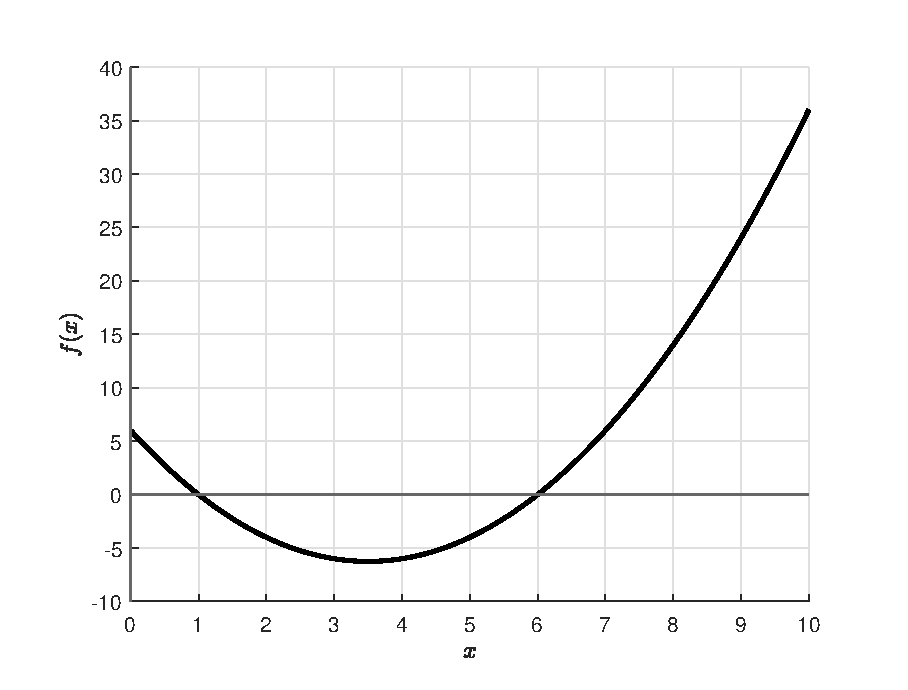
\includegraphics[width=250pt]{chapters/part5/figures/demo_problem_formulation.eps}
\caption{Plot of $f(x)=x^2-7x+6$} \label{fig:p5:onevarproblemformulation}
\end{figure} 